\chapter{Analisis}
\label{chap:analisis}

Bab ini membahas tentang analisis kebutuhan yang diperlukan oleh Teknik Informatika. Kebutuhan-kebutuhan tersebut didapat dari daftar isu repositori Sharif Judge di \textit{GitHub} dan dari para dosen pengguna Sharif Judge. Hasil dari analisis kebutuhan tersebut dicatat ke dalam Google Sheets dan didiskusikan dengan dosen pembimbing. Berikut hasil diskusi peniliti bersama dosen pembimbing yang dicatat ke dalam \textit{Google Sheets}. Selain analisis kebutuhan, pada bab ini juga akan dibahas solusi yang ditawarkan untuk memenuhi kebutuhan tersebut.

\begin{figure}[H]
	\centering  
	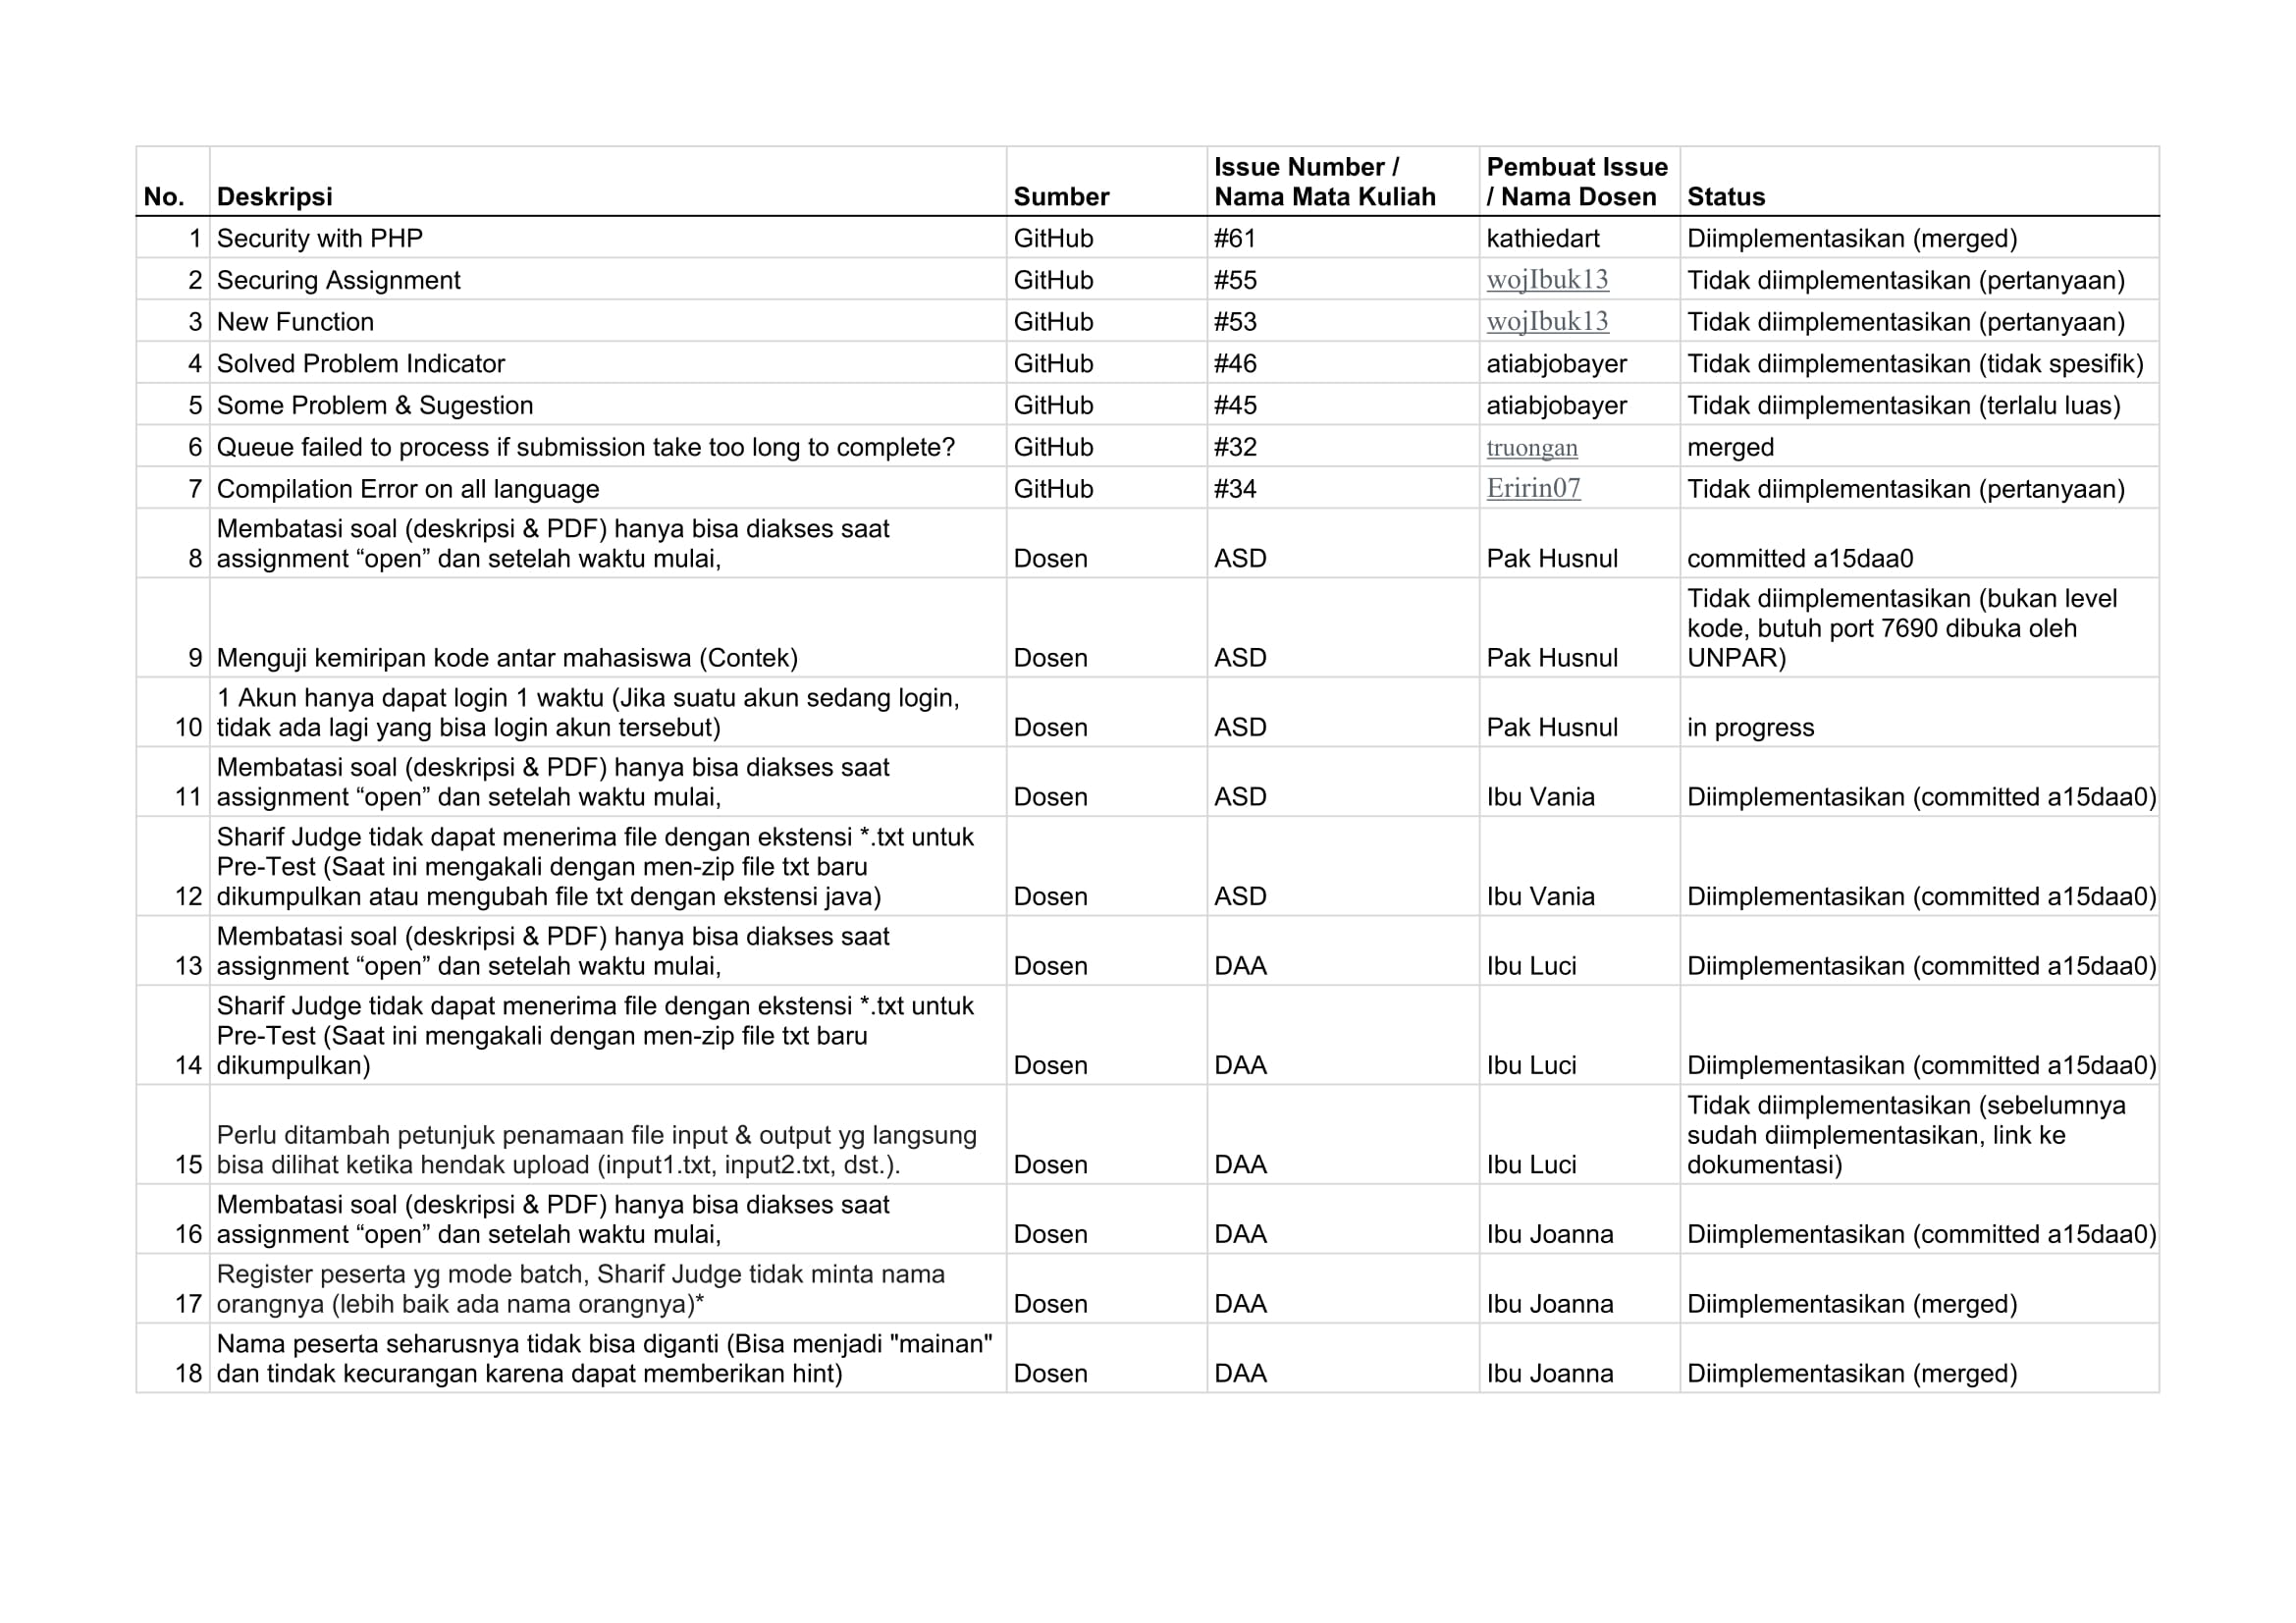
\includegraphics[scale=0.2]{pdf1}
	
	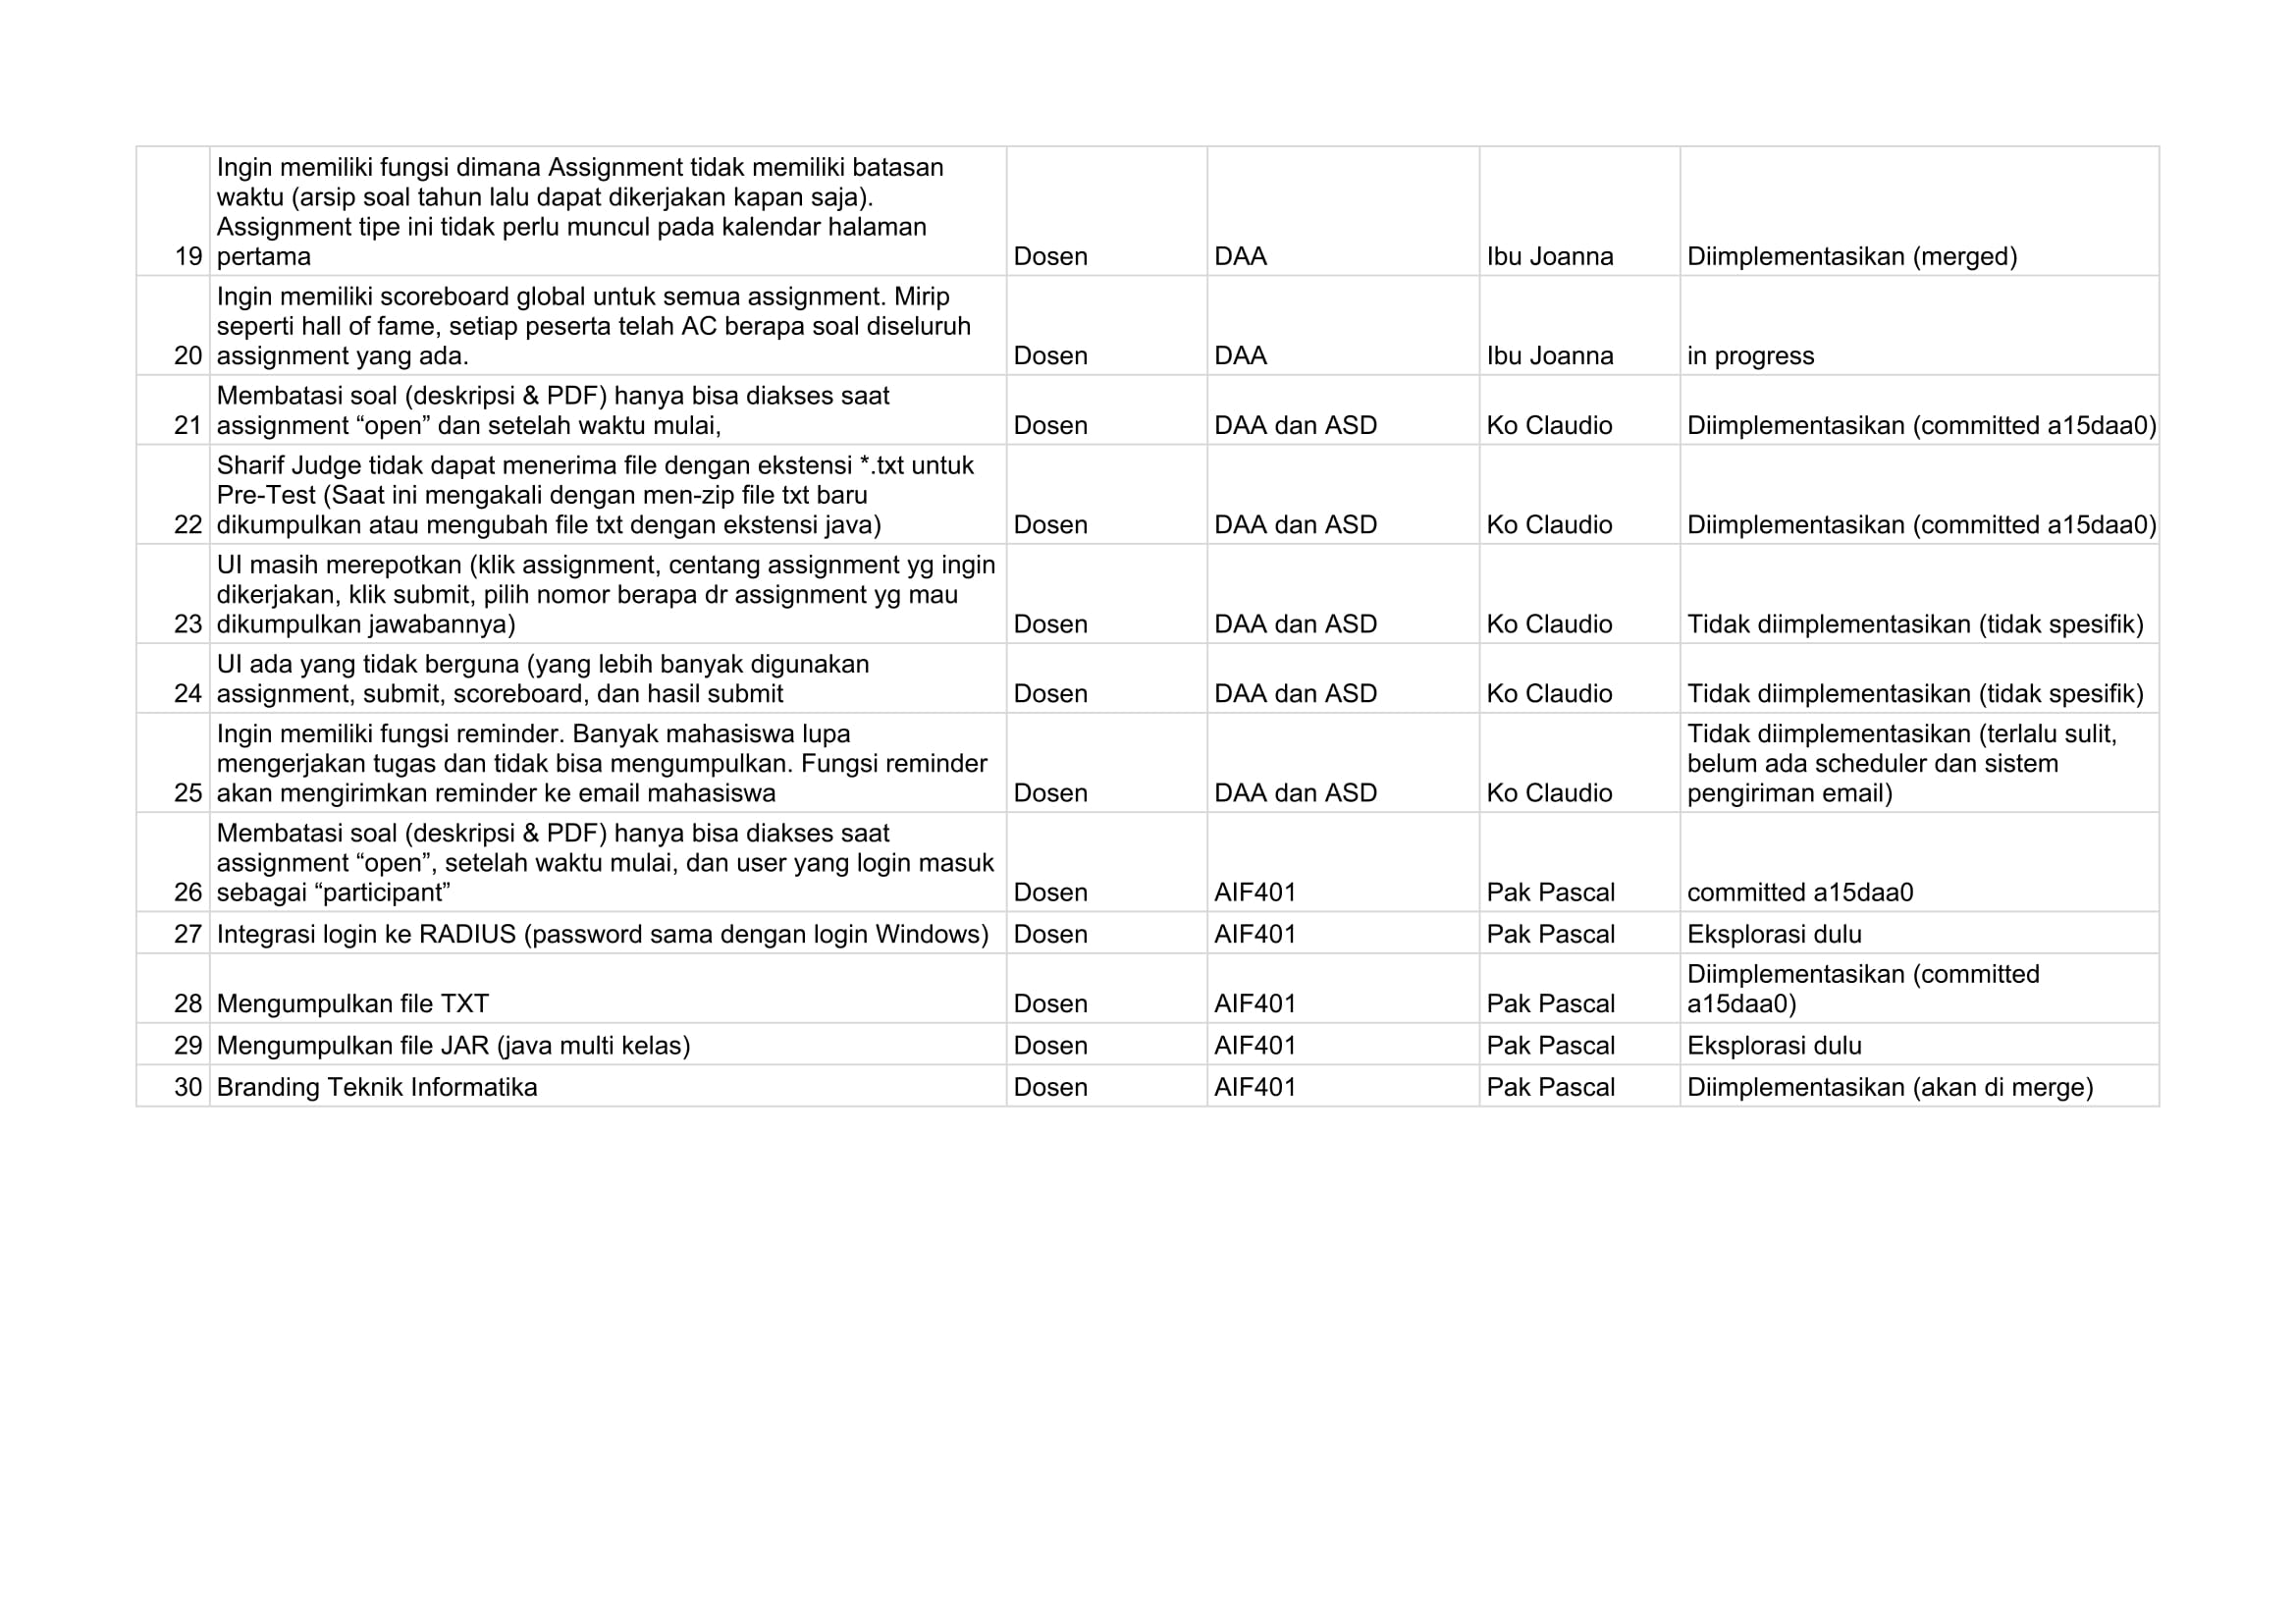
\includegraphics[scale=0.2]{pdf2}
\end{figure}

\section{Analisis Kebutuhan dari Daftar Isu Repositori Sharif Judge di textit{GitHub}}
\label{sec:analisisgithub} 
Analisis dilakukan dengan menganalisa setiap isu terbuka yang ada pada repositori. Dari analisa setiap isu tersebut, didapatkan beberapa pertanyaan dan usulan pengembangan. Beberapa isu yang memiliki usulan pengembangan akan dijadikan pertimbangan untuk mengembangkan Sharif Judge.

\subsection{\textit{Security with PHP} footnote}
Isu ini dibuat oleh pengguna textit{GitHub} dengan username \textit{danwdart}. Pada isu tersebut dikatakan bahwa seseorang pengguna Sharif Judge dapat mengubah parameter PHP shell\_exec() yang mengakibatkan pengeksekusian kode bisa dilakukan secara sewenang-wenang. %Hal tersebut dapat dicegah dengan cara mengubah perintah shell\_exec("rm ...") dengan method \textit{unlink()}.
	
\subsection{\textit{Queue failed to process if submission take too long to complete? footnote}}
Isu ini dibuat oleh pengguna textit{GitHub} dengan username \textit{truongan}. Pada isu tersebut dikatakan bahwa assignment yang memiliki masalah dengan test case yang besar menyebabkan submission status menjadi pending. %Hal diatas terjadi disebabkan oleh koneksi database times out. Untuk mengatasi masalah tersebut diperlukan method reconnect database pada file \textit{Queueprocess.php}.

\section{Analisis Kebutuhan dari Dosen Pengguna Sharif Judge}
\label{sec:analisisdosen} 
Analisis kebutuhan dari para dosen pengguna Sharif Judge dilakukan dalam bentuk wawancara secara langsung dan melalui email. Dosen-dosen yang telah diwawancarai antara lain:
\begin{enumerate}
	\item Bapak Husnul Hakim
	\item Bapak Claudio Franciscus
	\item Ibu Vania Natali
	\item Ibu Luciana Abednego
	\item Ibu Joanna Helga
\end{enumerate}
Dari hasil wawancara didapatkan beberapa kebutuhan yang sama dari setiap dosen pengguna Sharif Judge. 

\subsection{Menguji kemiripan kode antar mahasiswa}
Perangkat lunak Sharif Judge terkini sudah memiliki fitur untuk menguji kemiripan kode antar peserta dengan menggunakan Moss. Untuk sekarang ini Moss tidak dapat digunakan, karena Moss membutuhkan port 7690 yang diblok oleh UNPAR. Oleh sebab itu, kebutuhan ini tidak diimplementasikan.

\subsection{Satu Akun hanya dapat login satu waktu}
Para peserta Sharif Judge dapat login menggunakan akunnya di beberapa komputer. Peserta yang mengetahui user dan password peserta lain dapat dengan mudah login ke Sharif Judge. Hal tersebut sering dijadikan celah bagi beberapa peserta untuk melakukan tindak kecurangan. Peserta yang sudah login menggunakan akun peserta lainnya dapat melihat dan menyalin kode yang telah dikumpulkan ke Sharif Judge. Tindak kecurangan ini sering terjadi pada saat kuis maupun ujian. Bapak Husnul Hakim menginginkan perangkat lunak Sharif Judge dimana akun para peserta hanya dapat login satu waktu. Jika sebuah akun telah login di satu komputer, maka akun tersebut tidak dapat login di komputer lainnya. Diharapkan dengan adanya fitur tersebut dapat menekan jumlah tindak kecurangan yang terjadi.

\subsection{Perlu ditambah petunjuk penamaan file input & output}
Dalam membuat sebuah assignment pada perangkat lunak Sharif Judge terdapat file test case yang harus disertakan. Terdapat beberapa ketentuan  saat menyertakan file test case. Beberapa ketentuan tersebut seperti struktur direktori dan penamaan dalam file test case. Pada halaman add assignment terdapat link menuju dokumentasi Sharif Judge di GitHub yang menjelaskan ketentuan dalam menyertakan file test case. Ketentuan tersebut harus terpenuhi agar sebuah assignment dapat berjalan dengan baik. Oleh sebab itu, kebutuhan ini tidak diimplementasikan.

%\subsection{UI masih merepotkan}

%\subsection{UI ada yang tidak berguna}

\subsection{Sharif Judge diharapkan memiliki fungsi reminder}
Setiap assignment pada perangkat lunak Sharif Judge memiliki batas pengumpulan. Jika assignment telah melewati batas pengumpulan maka para peserta tidak dapat mengumpulkan tugasnya. Banyak peserta sering kali lupa untuk mengerjakan assignment dan pada akhirnya melewati batas pengumpulan. Bapak Claudio Fransiscus menginginkan perangkat lunak Sharif Judge yang memiliki fitur reminder. Fitur reminder akan mengirimkan email ke setiap peserta yang berisikan peringatan bahwa ada assignment yang harus diselsaikan. Namun kebutuhan ini belum dapat diimplementasikan karena masih belum ada sistem scheduller dan tingkat kesulitan yang terlalu tinggi.

\subsection{Membatasi soal (deskripsi \& PDF) hanya bisa diakses saat \textit{assignment} "open" dan setelah waktu mulai}
Kebutuhan ini merupakan salah satu kebutuhan yang paling banyak disebut oleh para dosen pengguna Sharif Judge. Perangkat lunak Sharif Judge terkini masih belum dapat memenuhi kebutuhan diatas. Para peserta dapat mengunduh diskrpsi soal \& PDF sebelum waktu \textit{assignment} dimulai. Untuk menangani hal tersebut para dosen harus mengunggah file PDF tepat pada saat assignment dimulai.

\subsection{Mengumpulkan file dengan format TXT}
Pengumpulan file dengan format TXT dibutuhkan untuk \textit{Pre-test}. Perangkat lunak Sharif Judge yang sekarang hanya dapat menerima file C, C++, Java, Python 2, Python 3, Zip, dan PDF. Para peserta yang ingin mengumupulkan jawaban \textit{Pre-test}, harus terlebih dahulu mengubah ekstensi file menjadi Java atau mengkompres file ke dalam Zip.

\subsection{Pendaftaran peserta disertai dengan \textit{Display Name}}
Pendaftaran peserta ke dalam Sharif Judge terkini tidak disertai dengan \textit{Display Name}. Perangkat lunak Sharif Judge membutuhkan empat buah parameter untuk mendaftarkan peserta, yaitu username, email, password dan role. Setiap peserta yang berhasil didaftarkan masih belum memiliki \textit{Display Name}. Para peserta harus memasukan \textit{Display Name} masing-masing secara manual.

\subsection{Nama pengguna Sharif Judge seharusnya tidak bisa diubah}
\textit{Display Name} pada perangkat lunak Sharif Judge berfungsi sebagai identitas peserta. Selain itu, \textit{Display Name} juga dapat berfungsi sebagai nama yang muncul pada bagian Scoreboard. Sharif Judge yang terkini mengijinkan para peserta untuk mengubah \textit{Display Name} pada bagian Profile. Hal tersebut dapat dijadikan sebuah "mainan" dan tindakan kecurangan karena dapat memberikan hint untuk peserta lain.

\subsection{Sharif Judge diharapkan memiliki fungsi dimana assignment dapat dikumpulkan tanpa adanya batasan waktu}
Pada masa Pra UTS dan Pra UAS biasanya para dosen memberikan assignment sebagai bahan pembelajaran. Arsip-arsip soal ujian dan latihan tahun lalu akan dijadikan sebuah assignment yang dapat dikerjakan oleh para peserta. Assignment tersebut memiliki waktu pengumpulan yang cenderung lama. Para dosen menginginkan sebuah fitur dimana assignment tersebut tidak memiliki batasan waktu dan dapat dikumpulkan kapan saja.

\subsection{Integrasi login ke RADIUS}
%Radius merupakan kependekan dari Remote Authentication Dial In User Service, merupakan protokol jaringan yang menjalankan service management Authentication, Authorization, dan Accounting (AAA) secara terpusat untuk user yang terkoneksi dan hendak menggunakan resource dalam jaringan footnote here
Lab FTIS UNPAR memiliki server RADIUS yang dapat memverifikasi ID mahasiswa terhadap kata sandinya. Integrasi Sharif Judge dengan RADIUS bertujuan agar para peserta dapat login ke Sharif Judge menggunakan akun yang terdapat pada server RADIUS.

\subsection{Branding Teknik Informatika}
Mengubah logo dan ikon Sharif Judge menjadi logo Teknik Informatika.

\subsection{Sharif Judge diharapkan memiliki Scoreboard global untuk semua assignment}
Sharif Judge terkini memiliki fitur Scoreboard yang berfungsi menampilkan seluruh nilai akhir para peserta dari sebuah assignment. Para dosen menginginkan sebuah Scoreboard global untuk semua assignment. Scoreboard global tersebut akan menampilkan berapa problem yang telah dikerjakan para peserta diseluruh assignment yang ada.

\subsection{Mengumpulkan file JAR (java multi kelas)}
